%%%%%%%%%%%%%%%%%%%%%%%%%%%%%%%%%%%%%%%%%%%%%%%%%%%%%%%%%%%%%%%%%%%%%%%%%%%%
% AGUJournalTemplate.tex: this template file is for articles formatted with LaTeX
%
% This file includes commands and instructions
% given in the order necessary to produce a final output that will
% satisfy AGU requirements, including customized APA reference formatting.
%
% You may copy this file and give it your
% article name, and enter your text.
%
%
% Step 1: Set the \documentclass
%
%

%% To submit your paper:
\documentclass[draft]{agujournal2019}
\usepackage{url} %this package should fix any errors with URLs in refs.
\usepackage{lineno}
\usepackage[inline]{trackchanges} %for better track changes. finalnew option will compile document with changes incorporated.
\usepackage{soul}
\usepackage{natbib}
\usepackage{amsmath}
\def\permille{\ensuremath{{}^\text{o}\mkern-5mu/\mkern-3mu_\text{oo}}}
\usepackage{lmodern}
\usepackage{float}

% DELETE this part
\usepackage{xargs}
% DELETE up to here

\linenumbers
%%%%%%%
% As of 2018 we recommend use of the TrackChanges package to mark revisions.
% The trackchanges package adds five new LaTeX commands:
%
%  \note[editor]{The note}
%  \annote[editor]{Text to annotate}{The note}
%  \add[editor]{Text to add}
%  \remove[editor]{Text to remove}
%  \change[editor]{Text to remove}{Text to add}
%
% complete documentation is here: http://trackchanges.sourceforge.net/
%%%%%%%

\draftfalse

%% Enter journal name below.
%% Choose from this list of Journals:
%
% JGR: Atmospheres
% JGR: Biogeosciences
% JGR: Earth Surface
% JGR: Oceans
% JGR: Planets
% JGR: Solid Earth
% JGR: Space Physics
% Global Biogeochemical Cycles
% Geophysical Research Letters
% Paleoceanography and Paleoclimatology
% Radio Science
% Reviews of Geophysics
% Tectonics
% Space Weather
% Water Resources Research
% Geochemistry, Geophysics, Geosystems
% Journal of Advances in Modeling Earth Systems (JAMES)
% Earth's Future
% Earth and Space Science
% Geohealth
%
% ie, \journalname{Water Resources Research}

\journalname{Geophysical Research Letters}

\hfuzz=100pt
\hbadness=10000

\begin{document}

%% ------------------------------------------------------------------------ %%
%  Title
%
% (A title should be specific, informative, and brief. Use
% abbreviations only if they are defined in the abstract. Titles that
% start with general keywords then specific terms are optimized in
% searches)
%
%% ------------------------------------------------------------------------ %%

\title{Sea ice heterogeneity as a result of ocean eddy activity during the ice growth season}

%% ------------------------------------------------------------------------ %%
%
%  AUTHORS AND AFFILIATIONS
%
%% ------------------------------------------------------------------------ %%

\authors{Josu\'e Mart\'inez-Moreno\affil{1}, Camille Lique\affil{1}, Claude Talandier\affil{1}}


\affiliation{1}{Laboratoire d'Oc\'eanographie Physique et Spatiale (LOPS), University of Brest/IFREMER/IRD/CNRS, Brest, France}

\correspondingauthor{Josu\'e Mart\'inez-Moreno}{josue.martinezmoreno@univ-brest.fr}

\begin{keypoints}
\item Mesoscale ocean eddies imprint heterogeneity on sea-ice thickness during the freezing season.
\item Eddies induce heterogeneity in sea-ice thickness by locally changing heat and salt fluxes at the ice-ocean interface. 
\item An increase in eddy field intensity leads to an increase in sea ice heterogeneity.
\end{keypoints}


\begin{abstract}
    Mesoscale eddies, generated by lateral gradients in salinity and temperature in the Arctic marginal ice zone, are known to modulate the melting of sea ice. Yet, it remains unclear if eddies modify sea ice growth during the freezing season. Here, we use idealized spin-down simulations of a front to explore the sea ice growth above an eddying ocean. In the presence of eddies, mixing of the sea surface temperature and salinity induces spatial variability in the heat and salt fluxes at the ice-ocean interface, imprinting spatial variability on the sea ice thickness. Sea ice thickness shows an order of magnitude more spatial variability in our simulations with strong eddies compared to those without. Increased spatial heterogeneity in the sea ice could make it more brittle and affect its evolution. This effect may become more pronounced as the Arctic transitions to a summer open-ocean regime and the eddy field intensifies.
\end{abstract}

\section*{Plain Language Summary}
\noindent Lateral variations of salinity and temperature in the Arctic Ocean caused by the melting or freezing of ice can result in ocean eddies (vortex-like features up to $\sim100$km in size). Previous studies have focused on how these eddies affect sea ice melting. However, it is not clear if eddies also play a role when the ice forms. Here, we use numerical simulations to see how these eddies influence the growth of sea ice. Eddies affect the temperature and salinity distributions at the ocean surface, which, in turn, modulate the thickness of sea ice as it forms. This eddy effect in the sea ice is important because it could impact the transitional zone between the open ocean and ice covered Arctic. Understanding these eddy-sea ice interactions is crucial to better understand the current and future states of the Arctic sea ice as it transitions to a summer ice free ocean.

\section{Introduction}\label{sec1}

The Arctic sea ice thickness varies over spatial and temporal scales ranging from a few meters to hundreds of kilometers and from days to several years \citep{Lewis_motion_1998, Mcnutt_spatial_2003}, making sea ice fundamentally heterogeneous \citep{Webster_ice_2022}. On one hand, large-scale variability ($\mathcal{O} > 100$km) in sea ice thickness is driven by the atmospheric forcing and large-scale ocean dynamics \citep{Mcnutt_spatial_2003,Morison_relaxation_2006,Halloran_drivers_2020}. 
On the other hand, the spatial and temporal variations at small scales ($\mathcal{O} < 100$km) are dictated by atmospheric synoptic processes \citep{Aue_cyclone_2022}, lateral heat transport by eddies between the open ocean and ice-covered areas, and local sea ice advection by eddies once ice is formed \citep{Cassianides_eddy_2021,Gupta_melt_2020,Horvat_ice_2018}. 
However, the spatial variability in sea ice conditions arising from oceanic eddies as the sea ice grows is yet to be fully characterized.

Eddies have been observed across the Arctic Ocean since the 1980s \citep{Johannessen_eddy_1987, Manley_eddies_1985}. Eddies are particularly prominent in the Marginal Ice Zone (MIZ), the region of transition between ice-free and ice-covered conditions characterized by sea ice concentrations between 15 and 80\% \citep{Kozlov_eddies_2020}. This is because the MIZ is also characterized by large lateral surface temperature and salinity gradients, which fuel the generation of instabilities resulting in the formation of eddies  \citep{Brenner_front_2020, Manucharyan_Ice_dynamics_2017, Lu_mixing_2015}. 
Eddies in the Arctic range from a few hundred meters to tens of kilometers (submesoscale - mesoscale ranges). They can have a significant influence on the local mechanical and thermodynamical behavior of sea ice, particularly in the MIZ \citep{Footprints_Manucharyan_2022}, where they can locally modulate heat transport and vertical heat flux under sea ice, and thus sea ice melt rates \citep{Appen_submesoscale_2018, Cassianides_eddy_2023}. Since there is a limited amount of in situ observations of the eddies under sea ice, many studies have used idealized simulations to better understand sea ice-eddy interactions. Some of these studies have shown the critical role eddies play in the melting of ice through the entrainment of warm subsurface waters into the mixed layer (ML), enhanced Ekman-induced vertical motion of warm waters to the surface, and lateral mixing and advection of warm waters below sea ice \citep{Gupta_melt_2020, Horvat_ice_2018, Manucharyan_Ice_dynamics_2017}. While these studies have focused on the effect ocean eddies have on sea ice melting, here we focus on the role eddies have in sea ice growth over the freezing season and their capacity to generate sea ice heterogeneity, specifically the spatial variability of the sea ice thickness. 

Oceanic eddies are present during both the melting and freezing periods of the sea ice \citep{Cassianides_eddy_2021, Kozlov_eddies_2020, Manucharyan_Ice_dynamics_2017}. In ice-free conditions, the Arctic Ocean can experience large heat and momentum exchanges with the atmosphere, thus, the eddy field can be energized. Furthermore, during the melting period, the stratification is weaker and the ML is shallow, in contrast to stronger stratification and deeper ML during the freezing period. This deepening of the ML can entrain subsurface waters, impact the sea-ice growth rates, and produce density anomalies that can generate turbulence and energize the eddy field. 
At the beginning of the freezing season, the sea ice thickness of a high resolution pan-Arctic hindcast (SEDNA; \citealt{SEDNA_2023}) is characterized by numerous eddies and filaments with scales characteristic of oceanic eddies (Fig. \ref{fig:fig1}a). 
Such features are up to 100 km wide, persist for several days (Fig. \ref{fig:fig1}d, e, and f) and match the similar mesoscale and submesoscale eddies visible in the sea surface salinity (SSS; Fig. \ref{fig:fig1}b) and sea surface temperature (SST; Fig. \ref{fig:fig1}c). These patterns and heterogeneity in the sea ice thickness are linked to a combination of atmospheric and oceanic processes during the sea ice freezing period, such as advection of sea ice by winds and ocean currents, spatially variable surface fluxes, and stirring by eddies. Since all of these processes are coupled, our approach is to isolate the heterogeneity driven solely by eddies (i.e. the heterogeneity induced by the advection of sea ice and heterogeneity in the surface fluxes due to eddies), in order to quantify the imprint of the ocean mesoscale activity on the sea ice conditions during at the Arctic freeze-up. 

\begin{figure}
    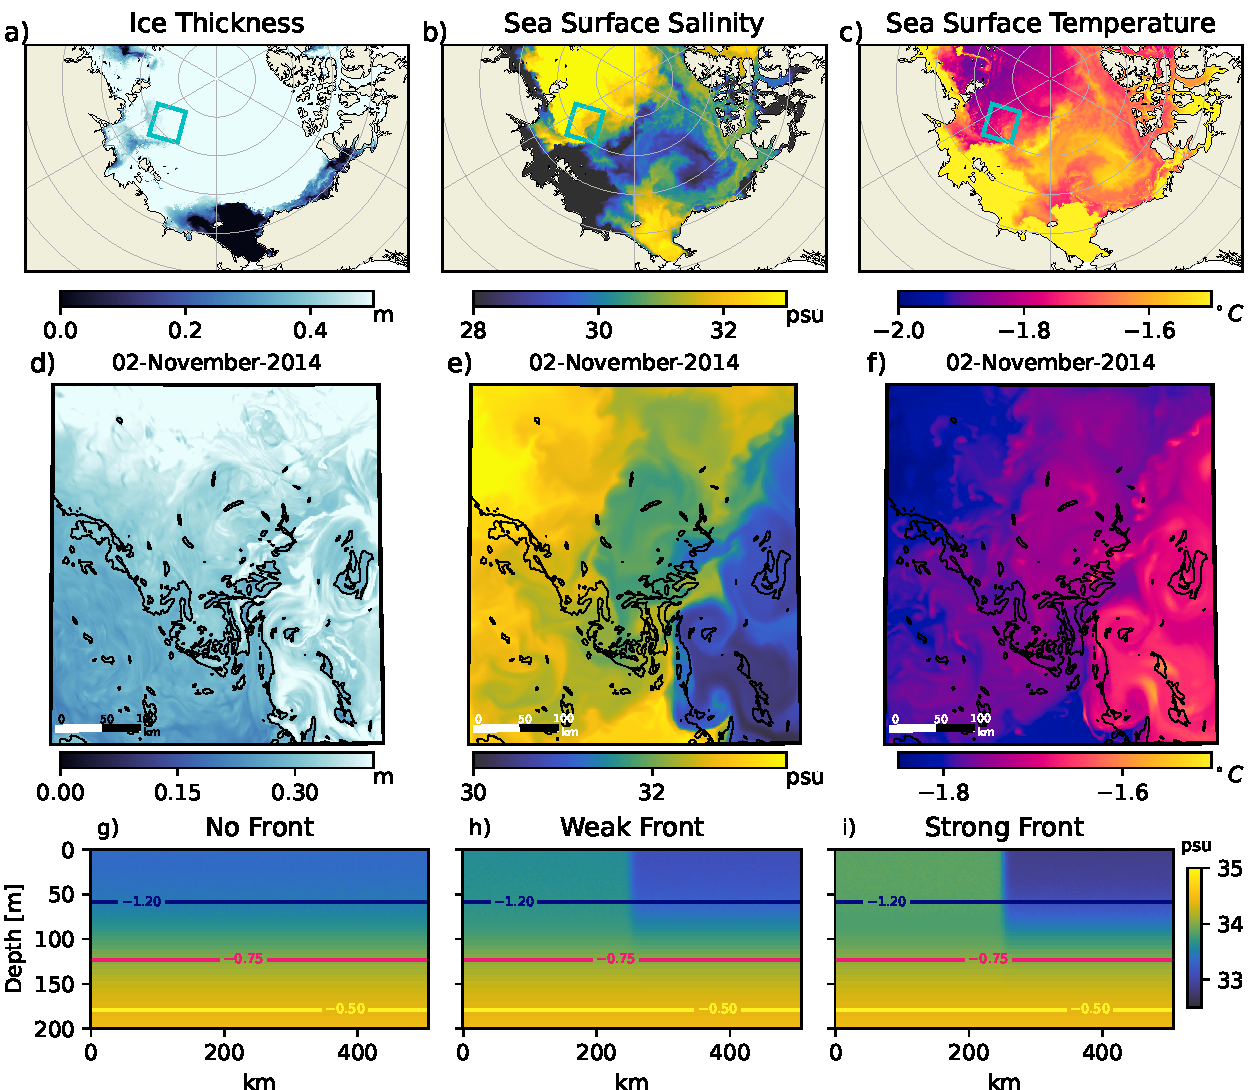
\includegraphics[width=1\textwidth]{Fig_1_combined_new.pdf}
    \caption{Snapshot of a) sea ice thickness (m), b) sea surface salinity (psu), and c) sea surface temperature ($^\circ$C) on  November 2, 2014 from SEDNA. Panels d, e, and f show two snapshots of the same quantities zoomed in the Laptev Sea (cyan box in panels a-c). In panels d, e, and f, the contours show the 80\% ice concentration. The initial salinity and temperature for the set of idealized configurations are shown in g) no front, h) weak front, and i) strong front. The background color corresponds to the salinity and contours show the temperature of each simulation. }
    \label{fig:fig1}
\end{figure}

\section{Methods}
\label{sec:Methods}

The present study uses a set of idealized channel configuration based on the NEMO modeling framework \citep{NEMO_man} fully coupled with sea ice model (SI3; \citealp*{SI3_man}). The sea-ice model uses an Elasto-Visco-Plastic (EVP) rheology with a 5-categories sea ice thickness distribution. The idealized simulations consist of a zonally reentrant channel that spans 1000 km zonally, 500 km meridionally, and 800 m in depth. The horizontal resolution is 2 km and the vertical has 100 levels with variable spacing that increases from 0.5 m at the surface to 18 m at the bottom. This resolution was chosen to resolve mesoscale features arising from baroclinic instabilities prescribed in the initial conditions. To limit the length scales of the flow, a logarithmic bottom drag is implemented. The Rossby radius across all three simulations is $\sim 10\ \mathrm{km}$, comparable to those found in the Arctic Ocean \citep{Nurser_rossby_2014}, and fully resolved by the model resolution. We use an $f$-plane approximation at around 80$^\circ$N, a scale-aware velocity dependent bi-harmonic isopycnal tracer diffusivity, and a bi-harmonic horizontal viscosity. The vertical mixing is based on the turbulent kinetic energy closure from \citet{blanke_TKE_1993}. A nonlinear equation of state is used to compute density (EOS80; \citealt{EOS_80}). The simulations are forced by a spatially constant daily climatology of shortwave and longwave radiations, and air temperature from ERA5 over the period 1979 to 2021 averaged north of 80$\mathrm{^\circ N}$. The fluxes between the ice-ocean-atmosphere are computed using the NCAR bulk formula \citep{Large_global_2009}. There is no wind forcing. 

We perform a set of three spin-down experiments to better understand the dependence of the ice on the presence and intensity of an eddy field. The first simulation (referred to as ``no front'') is initialized with horizontally uniform temperature and salinity fields. The vertical profiles of salinity and temperature are defined with a hyperbolic tangent, and resemble a characteristic winter profile of the Arctic, where salinity dominates the stratification ($\beta$-ocean; \citealp{Carmack_beta_ocean_2007}) and the halocline separates the fresher and colder ML from the saltier and warmer water below.
The structure of the initial conditions for all the simulations is shown in Figure \ref{fig:fig1}. The initial temperature profile is spatially constant in the 3 simulations. In the ``weak'' and ``strong'' front experiments, the salinity is redistributed meridionally to create a frontal structure of $\sim75\ m$ depth. This salinity redistribution preserves the same initial mean salinity across all simulations. The intensity of the front was chosen to match the typical SSS differences between the ice-covered region and the open ocean in the MIZ ($\sim1$ psu) found in the Arctic MIZ. The ``strong front'' experiment is initialized with this front, where fresh water covers the northern half of the domain (Fig. \ref{fig:fig1}i).
The ``weak front" experiment is analogous to the strong front, but the intensity of the salinity front is scaled by a factor of 0.5 ($\sim0.49$ psu; Fig. \ref{fig:fig1}h). Our configuration is inspired by \citealt{Manucharyan_Ice_dynamics_2017}, but our forcing allows the migration of the ice edge meridionally and the transition from MIZ to ice pack once the domain is fully ice-covered.

All the idealized simulations are initialized on May 1st with a sea ice thickness of 1 m over the entire model domain. The temperature and salinity fields include noise in the top 75 m to seed baroclinic instability (Fig. S1). As the magnitude of the initial horizontal salinity gradient increases, the resulting eddy field is more energetic (Fig. S1).
The idealized simulations are run for two years and the analyses presented hereafter comprise the freezing season of the second year of the simulation between September and December. After a full seasonal cycle, the initial fronts develop rich eddy fields, allowing us to study the surface impact of eddies on the sea ice growth. 

\section{The role of eddies in the generation of sea ice heterogeneity}\label{subsec2}

As in SEDNA, the idealized simulations with eddies (weak and strong fronts) show a spatially heterogeneous sea ice thickness from September onwards (Fig. \ref{fig:fig2}). Here again, the newly formed sea ice resembles the eddying features at the ocean surface. 
On the 15th of September, the no front experiment shows a homogeneous temperature field approximately $1^\circ$C above the freezing point. At the same date, the other experiments (weak and strong fronts) show a pronounced SST meridional gradient, where the northern part of the domain is close to the freezing point and the southern part is around $1.5^\circ$C warmer than the freezing point. Indeed, despite the constant initial temperature profile, a frontal structure develops in the temperature field due to the interplay between the spatial variations of the freezing point, stratification, and ML depth imposed by the salinity frontal structure on the northern and southern halves of the domain.
As time progresses (successive rows of Fig. \ref{fig:fig2}), the SST in the no front experiment reaches the freezing point in a couple of days, and a homogeneous layer of ice forms, covering the full domain in one day (Fig. \ref{fig:fig2}a and e). In contrast, the weak and strong front experiments show an SST and ice thickness rich in eddying features, and sea ice takes up to 14 days to fully cover the domain, since sea ice forms earlier or later over the colder and warmer SST regions, respectively (Fig. \ref{fig:fig2}b, c, f, and g). Over time, sea ice thickness resembles these eddying features in the regions where the ocean surface has reached the freezing point. 
Time series of the spatial standard deviation (STD) of the SST deviation from the freezing point and the ice thickness ($T-T_f$; Fig. \ref{fig:fig2}d) show a gradual decline in the SST STD after the 15th of September, coinciding with an increase in ice thickness STD. In fact, once the SST reaches the freezing point for each experiment, the ice thickness reaches its maximum STD. For example, the strong front experiment, with $\sim 30$\% higher $T-T_f$ STD before ice forms results in $\sim 30\%$ more ice thickness STD compared to the weak front, and one order of magnitude when compared with the no front. 

\begin{figure}
    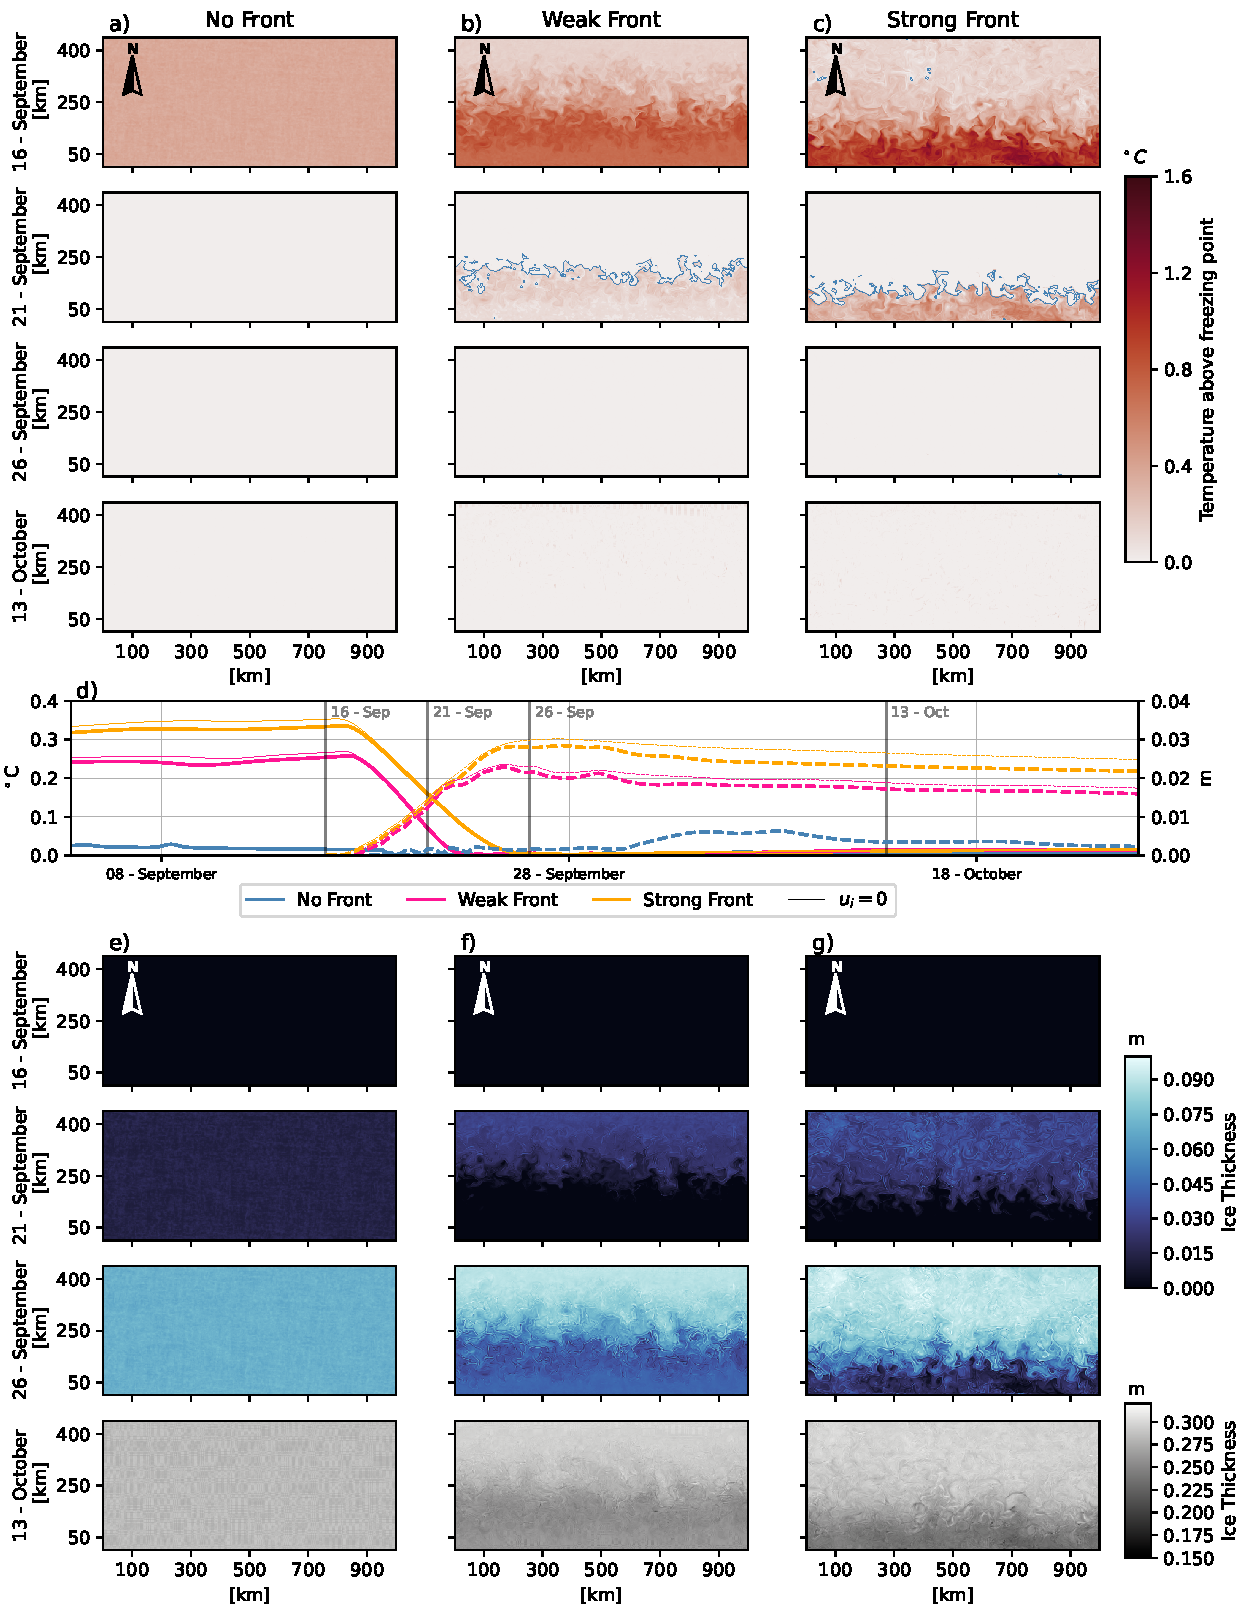
\includegraphics[width=1\textwidth]{Fig_2_combined_new.pdf}
    \caption{Snapshots of SST deviation from the local freezing point (a, b, and c, in $^\circ$C) and ice thickness (e, f, and g, in m) for the three idealized experiments. Each row show snapshots of on the 16th of September, 21th of September, 26th of September, and 13th of October for each experiment: no front a) and e), the weak front b) and f), and the strong front c) and g). The blue contours in panels b and c indicate the 0\% ice concentration and the north of the domain is indicated with the compass.
    Panel d) show the time-series of the STD of the temperature above the freezing point (solid lines) and ice thickness (dashed lines) for the different experiments. Thin lines corresponds to the weak and strong experiments imposing ice velocity to zero. } 
    \label{fig:fig2}
\end{figure}

The forcing of our idealized simulations does not include winds, nor any spatial heterogeneity in the atmospheric conditions.
Thus, the ice thickness variability in our simulations can only arise from ocean heterogeneity and/or sea ice advection after sea ice has formed. In order to quantify the relative contributions of these two processes, a modified version of the weak and strong front simulations is performed, in which the ice velocities are set to zero to remove the heterogeneity resulting from sea ice advection by eddies. These experiments show similar $T-T_f$ and ice thickness STD compared to the weak and strong front simulations (thick vs thin lines in Fig. \ref{fig:fig2}d), indicating that the primary source of heterogeneity arises from variations in SST and SSS during sea ice growth, rather than the advection by eddies of newly formed ice.

The spatial variability of SSS and SST, quantified by time-series of their spatial STD and their spectral variance, describes the magnitude and length-scales of the heterogeneity in the ocean surface capable to modify the ice growth and its heterogeneity. The STD of SST, SSS, and ice thickness are shown in Figure \ref{fig:fig3} for each experiment. 
There is a large variation of the STD magnitude of SST, SSS, and ice thickness across experiments. The no front experiment shows, across all diagnostics, a negligible STD averaged between the 15th of September and the 15th of October. In other words, there is a homogeneous response of the ice thickness and ocean surface properties. During the ice growth period, sea ice in the no front simulation behaves as a slab of ice, and an increase in sea ice thickness results in a spatially constant SSS increase due to a homogeneous brine rejection across the domain.
The weak front experiment exhibits a larger mean STD than the no front experiment of $0.02$ m in ice thickness, $0.02\mathrm{^{\circ}C}$ in SST, and $0.3$ psu in SSS (Fig. \ref{fig:fig3} and S2) over the same period.
Finally, the experiment with a strong front has the largest time-mean STD in ice thickness ($0.03$ m), SST ($0.03\mathrm{^{\circ}C}$), and SSS ($0.4$ psu). Note that the difference between the SST STD in the weak and strong experiments decreases rapidly over a few days because the ML is cooled down by the atmosphere until it reaches the local freezing point. Moreover, the SSS STD shows a rapid decrease over time, but the strong front retains $\sim 30\%$ more spatial variability than the weak front experiment. Overall, the different experiments reveal that the heterogeneity of ice thickness is larger in the presence of a stronger eddy field. 

The Hovm\"oller spectra of the SST, SSS, and ice thickness in figure \ref{fig:fig3} d, e, and f is computed by averaging the power spectral density of each zonal spectra of each field (along the periodic direction). The power spectral density of the SST, SSS, and ice thickness show that most of the variance is found within the mesoscale range ($R_D$-$2\pi R_D$; with $R_D$ the Rossby radius). Furthermore, the magnitude of the spectral variance increases by one order of magnitude between the no front and the weak front experiment and by another order of magnitude between the weak front and strong front. During the open-water ice-growth period, the SST and SSS spectral variance is distributed across a large range of spatial scales, but the maxima is within the mesoscale range (Fig. \ref{fig:fig3} e and f). Large spectral variance in the SST only lasts for the first couple of weeks of the open-water ice-growth period, after which it decreases two orders of magnitude and maintains a larger variance around the mesoscale scales. 
The SSS and ice thickness spectral variance in the weak front run is mostly contained within the mesoscale range of motions, while in the stronger front run, there is also a second peak of variance of SST and ice thickness at a larger scale ($\sim 200km$). These two length-scales result from the advection and mixing of tracers by eddies and the meridional meandering of the front, consistent with the spatial distribution of properties of a frontal region in the Laptev Sea in SEDNA (Fig. S3). However, the STD in SEDNA is larger since there are extra sources of heterogeneity (winds, latent and sensible fluxes, and others). Despite the influence of the meandering front, the presence of eddies makes the formation of ice spatially variable and the spatial length scale of the sea ice resembles the ocean mesoscale length scale. 

In December, several months after the domain is fully ice-covered and it has transitioned from a MIZ into an ice pack regime, the strong front STD of SST, SSS, and ice thickness is 30\% larger than that of the weak front experiment (Fig. 3 and S3). The strong front experiment has the largest spatial variability and the initial heterogeneity imprinted in the sea-ice at the beginning of the season is retained over the winter season. SSS heterogeneity is sustained during winter, which induces variations in the freezing point and thereby modulates the heat and salt fluxes at the ocean-ice interface.

\begin{figure}
    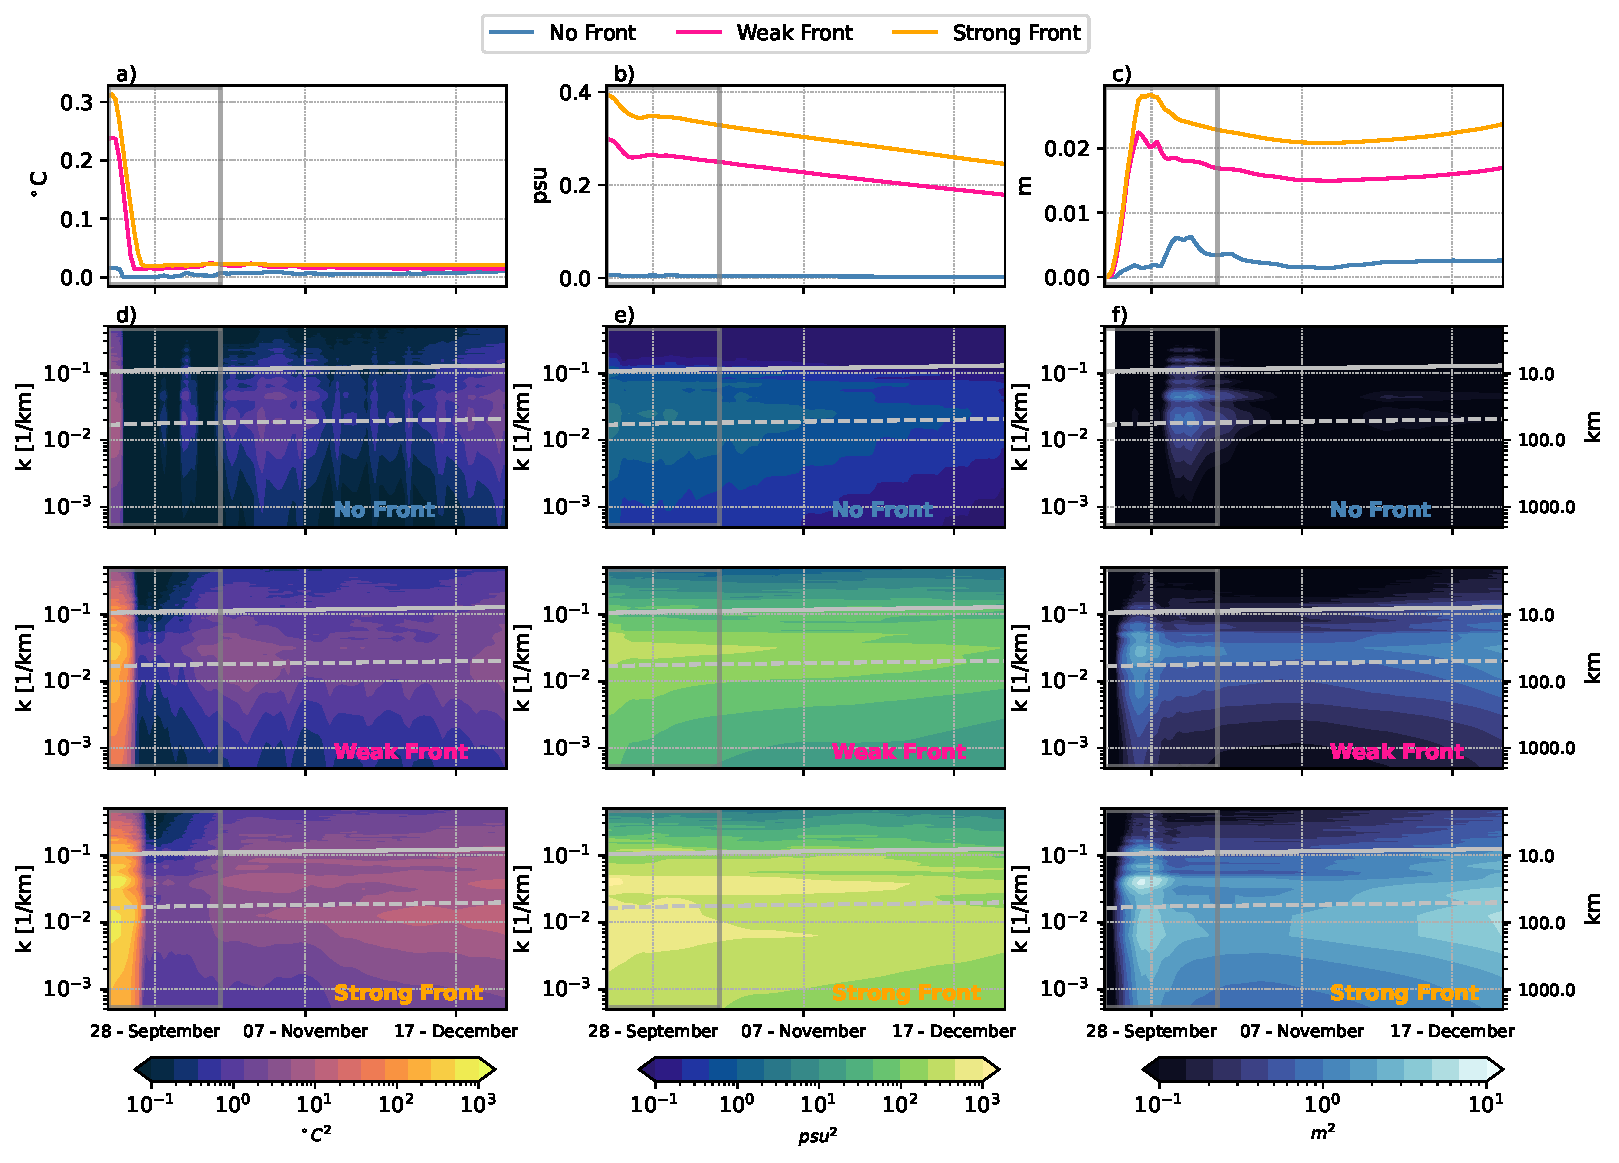
\includegraphics[width=1\textwidth]{Fig_3_STD_spectra_temp_salt_ice.pdf}
    \caption{Standard deviation time-series and Hovem\"oller diagrams of the power spectra of the SST, SSS, and ice thickness. SST, SSS, and ice thickness STD time series are shown in panel a, b, and c. Hovem\"oller of the power spectra of SST, SSS, and ice thickness for each experiment in d, e, and f, respectively. Rows in panels d, e, and f correspond to the no front, weak front, and strong front. Solid and dashed gray lines correspond to the mesoscale range ($R_D$-$2\pi R_D$). The gray box represents the open-water ice-growth period.}
    \label{fig:fig3}
\end{figure}

\section{The role of the ocean-ice flux in setting up ice heterogeneity}\label{subsec3}

At the beginning of the freezing season, the spatially heterogeneous ocean surface experiences cooling, and thus regions where the SST is at the freezing point use the additional heat flux lost to the atmosphere to grow ice. This is followed by brine rejection that increases the salt flux at the ice-ocean interface, and its effects are confined to the ML due to the strong stratification of the halocline. After sea ice has started to form, an increase in SSS lowers the local freezing point and creates a feedback loop of cooling and brine rejection. For example, in the strong front experiment the mean SSS on the 15th of September is $\sim31.3\text{ psu}$ and increases to $\sim32\text{ psu}$, on the 12th of October; this corresponds to a $\sim0.04^\circ\text{C}$ decrease of the freezing point. This ice-ocean feedback in the presence of eddies produces a spatially variable freezing point under the ice that sustains spatially variable heat and salt fluxes at the ocean-ice interface throughout the freezing season. 

The heat and salt fluxes at the ice-ocean interface depend on the mechanisms of sea ice growth: basal growth, new ice formation in open ocean, and snow ice formation. Since the experiments exclude snow processes, the only fluxes during the freezing period are the open water formation and basal growth. The open water heat and salt fluxes (Fig. \ref{fig:fig4}c and d) are different from zero when the ocean surface is in direct contact with the atmosphere and near the freezing point, at the beginning of the freezing season (15th of September). Figure \ref{fig:fig4}c and d shows that the STD of salt and heat fluxes in open water are only important during a short period ($\sim1$ month in October) and their spatial variability increases with the intensity of the front. For example, the time-mean STD of the open-water salt flux over the open-water ice-growth period is 5$\times10^{-8} \text{kg\ m}^{-2}\text{s}^{-1}$ for the no front experiment, 22$\times10^{-8} \text{kg\ m}^{-2}\text{s}^{-1}$ for the weak front experiment, and 27$\times10^{-8} \text{kg\ m}^{-2}\text{s}^{-1}$ for the strong front experiment (Figure \ref{fig:fig4}a). Analogous to the open water salt flux, the STD of the open water heat fluxes at the beginning of the freezing season is highly dependent on the ocean state. The no front experiment has the smallest STD of both the salt and heat fluxes since the full domain responds at the same time, however, some oscillations in the heat flux are visible since the absence of heterogeneity in this simulation results in a step-like growth. This pattern arises from the discrete deepening of the ML and the time required for atmospheric forcing to cool it down (Fig. \ref{fig:fig4}d). Over the open-water ice-growth period, the ice-ocean salt flux and heat fluxes from ice formation in open water in the strong front run are $\sim 20-25\%$ larger than those in the weaker front one. Thus the larger ocean tracer heterogeneity is transferred to the sea ice by fluxes at the ocean-ice interface.

\begin{figure}
    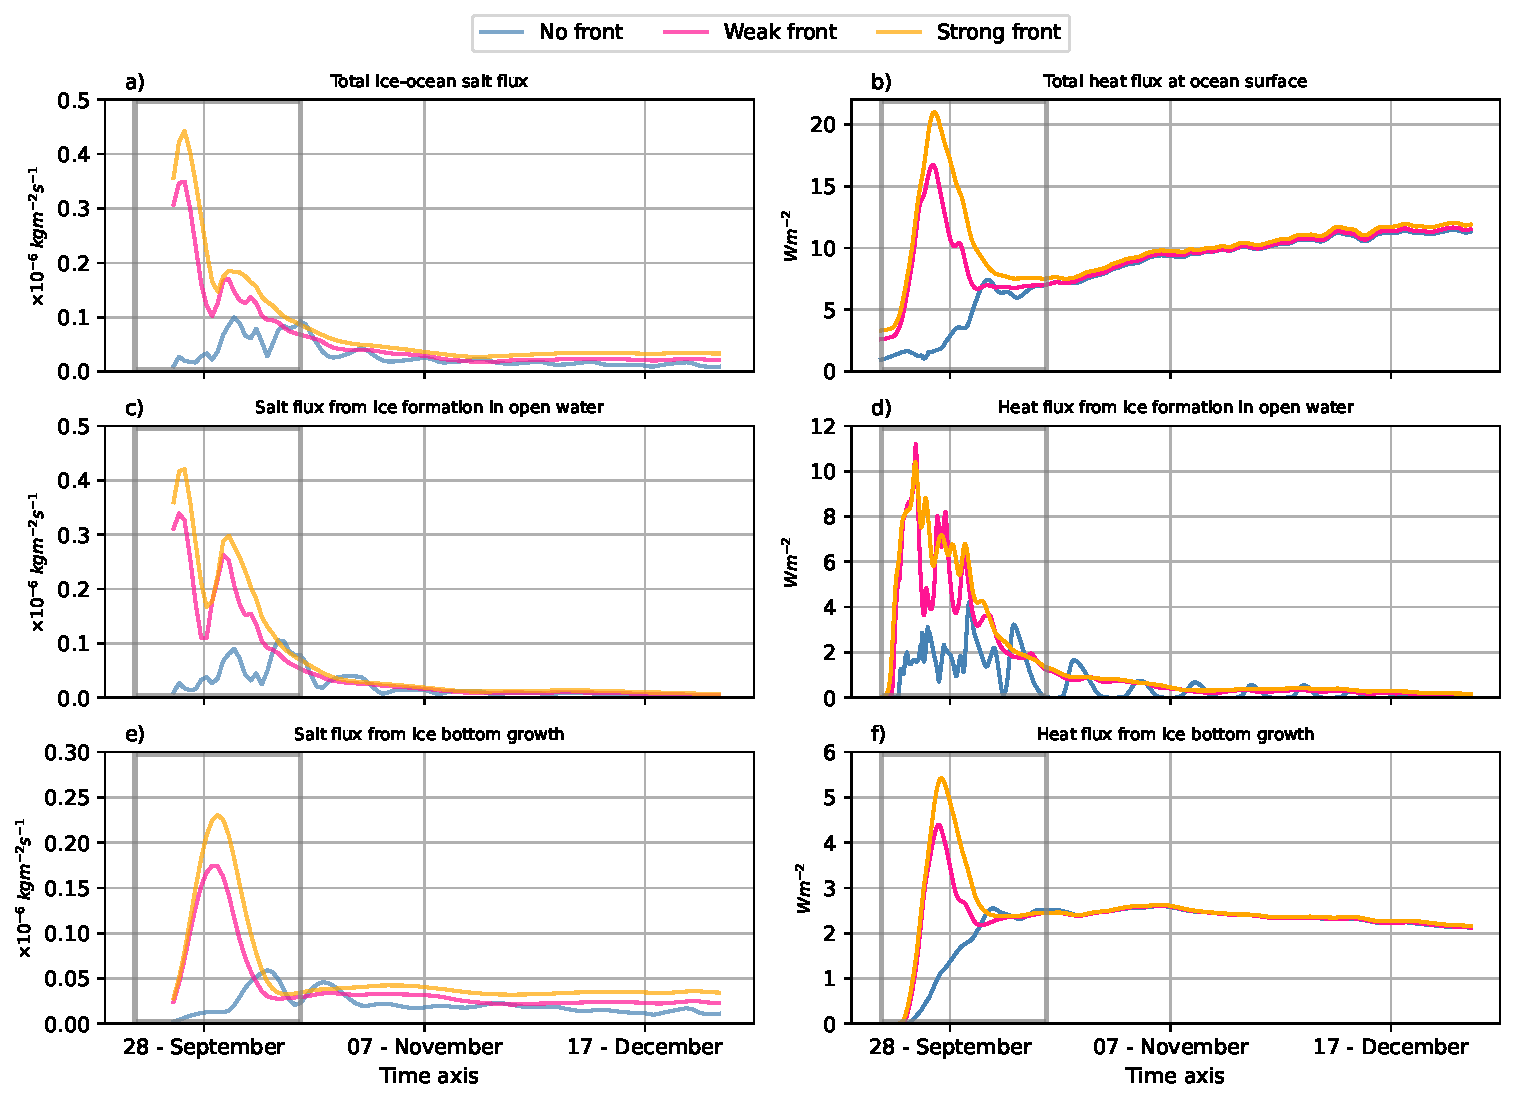
\includegraphics[width=1\textwidth]{Fig_4_mean_salt_heat_flux_expts_front_ts_relevant_std.pdf}
    \caption{Standard deviation of salt and heat flux and their major components for the three experiments. a) Total ice-ocean salt flux. b) Total heat flux at the ocean surface. c) Ice-ocean salt flux in open water. d) Heat flux used for open water ice formation. e) Ice-ocean salt flux from ice growth at the bottom.  f) Heat flux used for bottom ice growth. The gray box indicates the open-water ice-growth period.} 
    \label{fig:fig4}
\end{figure}

As the domain becomes partially or fully ice-covered, the largest fluxes at the ocean-sea ice interface correspond to basal growth. In our configuration, the transition between sea ice growth in open water to basal growth occurs on the 28th of September. Although the largest basal growth occurs in November, the STD of the salt flux from bottom growth is the largest in September and October with a small but distinct difference between simulation over the following months, where the STD of the strong front is 25\% larger than the weak front, and 70\% larger than the no front. The heat from ice bottom growth spatial STD is different across the simulations only in September and October (Fig. \ref{fig:fig4}e and f). 
After November, the STD of the basal growth heat fluxes are similar across all experiments at $\sim - 2.3 \text{Wm}^{-2}$. This behavior reveals that around one month after ice starts to grow, the heat fluxes become more homogeneous as the sea ice conditions become thicker and more concentrated. 
This result is consistent with the refreezing within the Laptev Sea in SEDNA (Fig. S4), as it takes approximately one month after sea ice starts to grow for the fluxes to become spatially homogeneous. 
The interplay between the fluxes from the open water and basal growth imprints the heterogeneity in the ice during the freezing season, emphasizing the critical role of ocean variability at the ice-ocean interface capable of imprinting heterogeneity in a short period of time, that lasts for several months in the sea ice. 

\section{Discussion and Conclusions}

The set of spin-down experiments, with varying intensities of the eddy field, shows an increase in the heterogeneity of sea ice depending on the intensity of the eddy field. Without eddies, ice formation is very fast, whilst, in the presence of eddies the ice formation starts a few days earlier, but it is slower lasting up to 14 days. Arctic eddies are known to laterally transport heat and salt \citep{Bashmachnikov_heat_transport_2023, Fine_Microstructure_2018}. Thus, mixing of SST and SSS by eddies, in addition to the ocean-atmosphere feedbacks responsible for determining the amount of ocean heat loss during the freezing season and the freezing point temperature, results in heterogeneous fluxes at the ocean surface that last several months after the freeze-up starts. In fact, advection of sea ice only plays a minor role imprinting the heterogeneity of the sea ice during the sea ice growth season, while heat fluxes appear to be the leading order driver of heterogeneity. Although ice thickness is more spatially heterogeneous in the presence of eddies, there is only a negligible difference in the total sea ice volume between the simulations, because the climatological atmospheric forcing (same in all the experiments) is the main forcing determining the sea ice volume at the end of the season. 

Our idealized simulations provide evidence that the ice can retain a memory of the ocean heterogeneity for several months after sea ice formation. This memory is stored in the sea ice during the freezing season and it is preserved as the ice transitions from a MIZ to ice pack dynamics. The STD of sea ice thickness before the following melting season is $\sim 30\%$ larger in the strong front than the weak front experiment (not shown). The persistence of heterogeneity with similar length scales to ocean mesoscale eddies (between $R_D$ and $2\pi R_D$) over the freezing season is likely to make the ice more brittle and prone to deform under atmospheric stress. It is interesting to note that the sea ice deformations observed by \citet{Rampal_sea_ice_2008} have a characteristic spatial scale of ~10 km. This scale is comparable to the eddy spatial scale and their imprint on sea ice through the mechanisms occurring at the time of sea ice formation, described here for the first time.
Thus, understanding the interactions between oceanic eddies and the sea ice is critical to better understanding variations of the Arctic sea ice conditions and their evolution.

The Arctic sea ice cover has declined dramatically since the 1990s due to the rapid warming of the Arctic, as a consequence of anthropogenic forcing \citep{IPCC_arctic_2022}. As ice cover is declining, the Arctic is transitioning towards a seasonally ice-free regime \citep{Crawford_open_water_2021}. Under this new paradigm, the ocean will experience a change in mechanical energy input and lateral temperature and salinity gradients at the ocean surface during ice-free seasons, resulting in an intensification of the ocean mesoscale and submesoscale fields \citep{Li_intensification_2024, Martin_trend_2014,McPhee_intensification_2013}. Our analyses suggest that doubling the intensity of the salinity front results in 30\% more spatial variability in sea ice thickness over the freezing season. Therefore, characterizing the impacts eddies have in the sea ice thickness heterogeneity is crucial to better represent the interactions between the ice and the ocean and likely to better understand the transition towards a more energetic summer ice-free Arctic. The current generation of climate models lacks the resolution to represent eddy-sea ice interactions in the Arctic, therefore, including these interactions could reduce the uncertainties associated with the prediction of climate change in the Arctic. 
 
Finally, our results show the importance of resolving the eddy field underneath forming sea ice. While the atmosphere is thought to be the main source of sea ice heterogeneity, here we show that eddies also play a role in setting up this heterogeneity. This eddy-driven heterogeneity is expected to occur in conjunction with other sources of heterogeneity, such as heterogeneity in the atmosphere, radiative fluxes, surface waves, entrainment of subsurface warm waters, and sea ice advection by winds. Thus, the relative importance of the eddy-induced heterogeneity discussed in this paper, and the feedback with other processes should be further explored. Missing processes such as winds, high-frequency forcing, and spatially varying radiative fluxes could energize the upper ocean and thus imprint further heterogeneity on sea ice \citep{Gupta_melt_2022}. Additionally, our study uses an Elasto-Visco-Plastic rheology that could impact the advection of the sea ice and thus the heterogeneity driven by eddies. However, we hypothesize that using discrete sea ice floes will likely result in similar results since floe growth will initially follow the heterogeneous freezing point stirred by the ocean eddy field. Our results focus on the Arctic Ocean, however, eddies in the Southern Ocean stand to impact the heterogeneity of the Antarctic sea ice through the same processes. Further research is required to describe and quantify the impact of eddies in high-resolution climate simulations, in addition to the joint impacts and contributions of eddies and winds in the heterogeneity of the Arctic sea ice and their preconditioning in the sea ice deformation.

\section{Open Research}

The idealized model configuration is described and publicly available at \citet{martinez_moreno_2023_10205736}. SEDNA, the high-resolution pan-Arctic model configuration is described and publicly available at \citep{SEDNA_2023}.
All analyses and figures in this manuscript can be reproduced using the Jupyter notebooks and instructions provided in the Zenodo archive \texttt{Ice\_formation}, \citet{josue_martinez_moreno_2024_13358894}.

\acknowledgments

We thank Till Wagner and the anonymous reviewers for their constructive feedback.
We thank Clement Rousset and Martin Vancoppenolle for their invaluable help with the numerical model. We also thank Anne-Marie Treguier and Angelina Cassianides for the constructive discussions that motivated some of the discussions described in the manuscript.
We acknowledge funding from the ANR ImMEDIAT project (ANR-18-CE01-0010) and the MEDLEY project funded by the program JPI Ocean/JPI Climate (ANR-19-JPOC-0001) project. The idealized simulations and their analysis were performed using the HPC facilities DATARMOR of ’Pôle de Calcul Intensif pour la Mer’ at Ifremer, Brest, France. We acknowledge PRACE for awarding computing time for SEDNA on the Joliot-Curie computer at GENCI\makeatletter@CEA, France.

\nocite{*}
\bibliography{biblio}

\end{document}